\chapter*{Les Mécanismes de la Coordination et l'Évolution de la Coopération :\newline {\Large de la Modélisation Computationnelle à la Conception en Robotique Évolutionniste} \newline \textit{\large Arthur BERNARD}}

\setcounter{chapter}{1}

\minitoc[n] % minitoc without title

\setcounter{page}{1}

\section{Résumé}

	Cette thèse porte sur l'utilisation des outils de robotique évolutionniste~\parencite{Nolfi2000, Doncieux2015a} pour l'évolution de la coopération de deux manières différentes. La première approche est une approche de modélisation computationnelle dont le but est d'étudier l'évolution biologique de la coopération mutualiste. La coopération est un comportement présent sous des formes très diverses et dans de nombreux taxa du vivant. Expliquer son évolution représente alors un défi majeur de la biologie évolutionniste. Notre but ici est d'utiliser la robotique évolutionniste pour enrichir les connaissances apportées par les modèles classiques utilisés en biologie évolutionniste. Nous voulons notamment nous intéresser à l'influence des mécanismes pratiques des comportements de coordination dans l'évolution de la coopération. Nous montrons notamment que prendre en compte ces mécanismes change drastiquement les prédictions faites par les modèles classiques. Notre seconde approche est de concevoir des systèmes multi-robots à l'aide de robotique évolutionniste. Ainsi, nous nous intéressons à cette méthode comme une manière de concevoir automatiquement le comportement de robots que l'on souhaite voir se coordonner. Plus particulièrement, nous nous intéressons à la qualité des comportements de coordination et à l'influence de la composition génétique des groupes de robots sur la nature de la coordination et la facilité de faire évoluer la coopération. Notre intérêt se porte notamment sur l'évolution de la division du travail parmis un groupe de robots hétérogènes.


\section{Introduction}

	\subsection{L'Abondance des Comportements Coopératifs}

		La coopération est un comportement qui se retrouve à toutes les strates de complexité du monde animal. Ses différentes formes sont variées et sont parfois centrales dans de nombreuses espèces. Strictement, la coopération est défini comme un comportement où un acteur (c'est-à-dire l'individu initiant la coopération) agit d'une manière qui est bénéfique à un destinataire~\parencite{West2007a}. Cette définition couvre donc un large éventail d'actions collectives.

		Nous pouvons trouver des exemples de coopération à presque tous les niveaux de complexité du vivant. Par exemple, des êtres unicellulaires tels que les bactéries sont connus pour fréquemment se comporter de manière coopérative. Ces organismes utilisent notamment des sécrétions afin de pouvoir partager des ressources et communiquer~\parencite{Elena2003}. Nous pouvons citer l'exemple particulier des \emph{Pseudomonas aeruginosas} qui sont capable de produire des nutriments que tout organisme voisin peut utiliser. Mais ce qui est particulièrement intéressant dans cet exemple est que produire ces nutriments est coûteux pour ces organismes. Ceci crée une situation complexe connue en biologie ainsi qu'en économie et appelée \emph{public goods games}~\parencite{Popat2012, Harrison2013}, que nous pourrions grossièrement traduire par \emph{dilemme des biens publics}. L'idée importante derrière ce terme est que ce genre d'acte de coopération est sensible à l'exploitation par des tricheurs. Ce terme ne traduit pas de jugement moral sur les comportements de ces individus mais permet simplement de transmettre l'idée que ces individus profitent des nutriments d'autres individus sans eux-mêmes en produire. C'est-à-dire qu'ils profitent des bénéfices de la coopération sans avoir à en payer le coût.

	  \begin{figure}[hbt]
	      \begin{center}
	        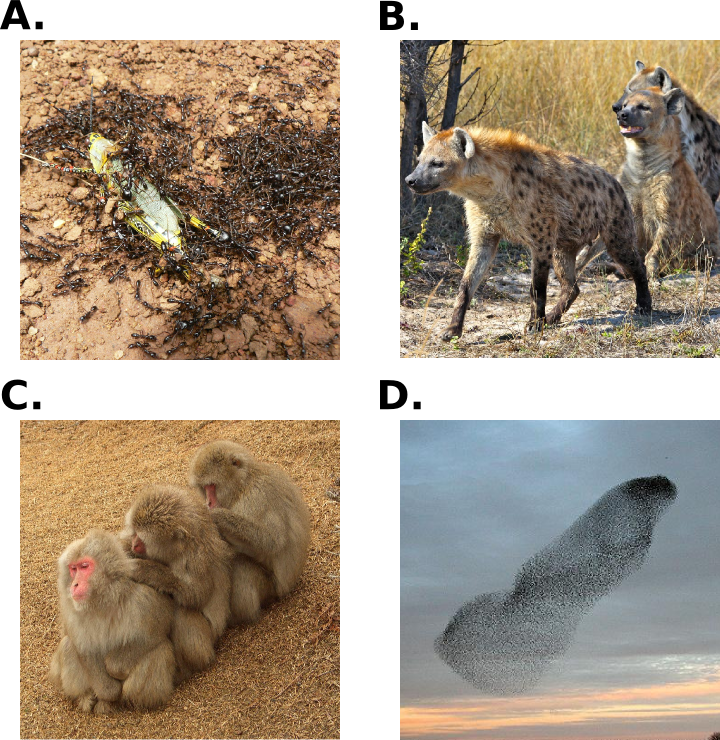
\includegraphics[scale = 0.5]{fig/Intro/CooperationExamples.png}
	        \caption{\textbf{La coopération à différents niveaux de complexité.} {\em (A)}~Les insectes eusociaux (comme les fourmis) possèdent une structure sociale extrêmement avancée. {\em (B)}~Les carnivores sociaux sont capables de coopération évoluée ainsi que de se coordonner durant des chasses collectives. {\em (C)}~Le toilettage social est une activité durant laquelle les individus se toilettent à tour de rôle. {\em (D)}~Les volées d'oiseaux montrent l'émergence de déplacements collectifs d'une manière qui laisserait penser que les individus ne font partie que d'une seule entité.} 
	        \label{fig:CooperationExamples}
	      \end{center}
	  \end{figure}

		Un autre célèbre exemple de coopération est celui des insectes \emph{eusociaux}~\parencite{Wilson1990} (voir Figure~\ref{fig:CooperationExamples}~(A)). L'eusocialité est une forme extrême de société qui se retrouve principalement chez les Hymenoptères (par exemple les fourmis, guêpes et abeilles) et Isoptères (notamment les termites). L'eusocialité est définie par des formes avancés de coopération. En particulier, le soin des jeunes est pris en charge de manière collective par d'autres individus qui ne sont pas leur parents. Les animaux eusociaux font aussi généralement preuve d'une forme avancée de division du travail, où les individus se partagent une tâche en se répartissant en plusieurs rôles. Enfin, et c'est une des caractéristiques principales de l'eusocialité, il y a aussi une division de la reproduction. Ceci veut dire qu'il existe des castes reproductives et non-reproductives.

		Nous pouvons aussi nous intéresser aux comportements coopératifs des vertébrés. En particulier, les carnivores sociaux sont capables d'actions collectives poussées. Ces espèces sont notamment souvent connues pour leurs comportements de chasse collective où plusieurs individus sont capables de se coordonner afin d'attraper ensemble une proie qu'un individu seul n'aurait pu chasser. Les hyènes tâchetées (Figure~\ref{fig:CooperationExamples}~(B)) par exemple usent de signaux de communication avancés afin d'être capable de pouvoir chasser ensemble~\parencite{Drea2009a, Smith2010, Smith2012a}. Mais elles vivent aussi dans des groupes sociaux très organisés où les femelles sont en haut de la hiérarchie. Les femelles dominantes sont généralement les seules à se reproduire tandis que les femelles de rang inférieur s'occupent du soin des jeunes des dominantes. Nous pouvons aussi faire référence aux primates, qui ont des structures sociales très poussées. Ces derniers s'engagent notamment dans du toilettage mutuel (voir Figure~\ref{fig:CooperationExamples}~(C)) entre différents individus du groupe~\parencite{Spruijt1992}.

		Enfin, à un niveau encore supérieur (en terme de taille), nous pouvons citer les comportements de déplacement collectifs, par exemple des volées d'oiseaux (Figure~\ref{fig:CooperationExamples}~(D)). De manière générales, de nombreux animaux différents peuvent s'organiser en volée, troupeau ou bancs d'individus~\parencite{Couzin2002, Couzin2003}. Ces comportements d'agrégation ont de nombreux avantages pour le groupe tels qu'augmenter la confusion d'un prédateur, diminuer le risque pour un individu en particulier d'être attaqué ou se défendre de manière collective.


	\subsection{L'Évolution de la Coopération}

		Malgré l'omniprésence de la coopération dans le monde animal, expliquer son évolution est un défi majeur en biologie évolutionniste.~\parencite{Hamilton1964, Dugatkin2002, West2011a}. En effet le principe de l'évolution tel que théorisé par Darwin peut être résumé par l'expression : "la survie du plus apte"~\parencite{Darwin1859}. Par conséquent, le comportement d'un individu ne peut être adaptatif que s'il lui est bénéfique. Plus précisément, le matériel génétique d'un individu se transmet lors de la reproduction. De là il ressort que, pour qu'un gène puisse se transmettre et donc se répandre dans la population, il est nécessaire qu'il permette à l'individu qui le possède d'augmenter sa capacité reproductive. Un trait particulier n'est donc adaptatif que s'il permet d'augmenter le nombre de descendants d'un individu (ce qu'on appelle valeur sélective ou plus généralement \emph{fitness}).

		C'est sur ce point que l'évolution de la coopération semble être une contradiction. En effet, par définition, un comportement coopératif apporte un bénéfice à un autre individu. Il est à noter qu'à partir de maintenant, lorsque nous ferons mention de bénéfices et coûts, nous nous référerons aux bénéfices et coûts à la valeur sélective des individus. C'est-à-dire que, lorsqu'un comportement est bénéfique à un individu, c'est qu'il permet \emph{au final} à cet individu d'accroître son nombre de descendants. Un comportement coopératif est donc un comportement qui augmente la fitness d'un autre individu. Parfois même, coopérer est coûteux (d'un point de vue de la valeur sélective donc) pour l'acteur. C'est par exemple le cas pour notre exemple précédent des \emph{P. aeruginosas}, pour qui sécréter des nutriments est coûteux. Cet exemple peut nous servir à mieux illuster le problème posé par l'évolution de la coopération. Imaginons une situation où des organismes coopèrent et sécrètent donc des nutriments qui peuvent être utilisés par tous. Imaginons maintenant qu'un mutant apparaît aléatoirement dans cette population et que ce mutant possède un trait qui le pousse à tricher plutôt que coopérer. Il va donc profiter des nutriments sécrétés par les coopérateurs sans lui-même produire ces nutriments et donc en payer le coût. Par conséquent, sa valeur sélective sera supérieure à celle des coopérateurs. Il va donc pouvoir produire plus de descendants et son génotype de tricheur va pouvoir se répandre dans la population. Ceci va continuer jusqu'à que la population ne soit plus composée que de tricheurs. Il apparaît donc que la coopération ne devrait pas être stable. De nombreux modèles ont donc été proposés afin de définir des mécanismes pour expliquer l'évolution de la coopération. Ces mécanismes peuvent être majoritairement classés en deux catégories: les bénéfices \emph{directes} ou \emph{indirectes} à la fitness~\parencite{West2007a}.

		Les bénéfices indirectes permettent notamment d'expliquer l'évolution de \emph{l'altruisme}. L'altruisme est un cas particulier de coopération dont nous avons précédemment parlé où coopérer est coûteux pour l'acteur du comportement coopératif~\parencite{Hamilton1964, West2007a}. Le comportement des \emph{P. aeruginosas} peut donc être considéré comme altruiste. La division de la reproduction chez les insectes eusociaux, où seule une certaine caste d'individus peut avoir des descendants est aussi un exemple d'altruisme. Les individus non-reproducteurs paient en effect le coût maximal puisqu'ils ne produisent pas de descendants du tout et ne peuvent donc pas transmettre leur matériel génétique. Il est donc difficile de comprendre comment un tel comportement peut être stable. Le mécanisme permettant d'expliquer l'évolution de l'altruisme a été proposé par Hamilton et s'appelle la \emph{sélection de parentèle}~\parencite{Hamilton1964}. Derrière ce terme est l'idée qu'un trait peut être transmis à travers les parents d'un individu. Si on considère en effet que l'unité de sélection est le gène, c'est-à-dire que l'évolution est due au fait qu'un gène permettant à un individu d'augmenter son nombre de descendants pourra ainsi se répandre dans la population, il n'est pas nécessaire que l'individu possédant ce gène se reproduise. En effet, s'il permet d'aider un individu qui est génétiquement proche de lui (un parent donc), il peut ainsi permettre à un gène permettant un comportement altruiste de se répandre aussi. La valeur sélective d'un trait n'est donc pas dépendante uniquement de la valeur sélective de l'individu possédant ce trait, mais aussi de celle de ces proches. C'est ce qu'on appelle la \emph{valeur sélective inclusive}. Ainsi un trait peut apporter des bénéfices indirectes en augmentant cette valeur sélective inclusive.

		Mais, tandis qu'un très grand nombre de travaux a été concentré sur l'évolution de l'altruisme et les bénéfices indirectes, la plupart des comportements coopératifs bénéficient directement à l'acteur. Dans ce cas, et l'acteur et le destinataire bénéficient du comportement coopératif. On parle aussi de comportement mutuellement bénéfiques pour cette catégorie de la coopération~\parencite{Bergmuller2007a}. Plusieurs mécanismes peuvent permettre d'expliquer comment la coopération peut-être adaptative grâce à des bénéfices directes. En particulier, ces bénéfices peuvent être forcés à travers de la réciprocité, des punitions ou encore des récompenses. Mais ces bénéfices peuvent aussi ne pas être forcés dans le cas où tous les individus partagent un intérêt à coopérer. Dans ce cas, on parle aussi parfois de \emph{bénéfices dérivés} afin de transmettre l'idée que la coopération peut-être dérivée d'un acte originellement égoïste. par exemple, faire partie d'un groupe plus grand d'individus permet d'augmenter les chances de survie (aussi bien face à l'environnement que contre des prédateurs) mais permet aussi de tirer des bénéfices plus importants de la chasse et de la récolte~\parencite{Clutton-Brock2002}. Une partie de la littérature sur la coopération mutuellement bénéfique s'intéresse aussi la coopération entre individus d'espèces différentes, ou coopération inter-espèces. Ceci s'appelle aussi du mutualisme (créant parfois une confusion avec le concept plus général de comportement mutuellement bénéfique). Par exemple, une certaine espèce de poissons, les Labres, sont connus pour le fait qu'ils nettoient d'autres poissons plus gros de leurs parasites et tissus morts. Mais de manière plus générale la coopération mutualiste intra-espèce est prédominante dans le monde animal. Et plus important, beaucoup de cas de coopération qui apparaissent altruistes à première vue sont en fait mutuellement bénéfiques. Par exemple, le Cratérope écaillé est un oiseau qui est connu parce que certains individus montent la garde et préviennent les autres de l'approche d'un prédateur, donnant ainsi l'impression qu'ils prenaient le risque d'être ainsi détecté par le prédateur en plus d'aider les autres à chercher de la nourriture. En véritié, le rôle de sentinelle est pris par des individus ayant déjà récolté suffisamment de nourriture et leur permet alors de maximiser leur propre survie dans un environment où les prédateurs sont nombreux~\parencite{Wright2001, Clutton-Brock2002}. Les comportement de coopération mutuellement bénéfiques sont donc cruciaux ainsi qu'à la base de la formation d'une structure sociale chez de nombreuses espèces.

		D'après ce que nous avons présenté précédemment, il pourrait apparaître que l'évolution de la coopération mutualiste est triviale. Et en effet, si on étudie uniquement le problème de la stabilité du comportement coopératif c'est le cas. Par exemple, comme expliqué avant, les comportements altruistes posent un problème de stabilité. Puisque ces comportements sont coûteux pour l'acteur, alors ils sont susceptible à l'invasion de tricheurs. Dans le cas des comportements mutuellement bénéfiques ce n'est plus le cas : puisqu'ils profitent à tous, un tricheur n'aurait aucun avantage à envahir la population. Cependant, ces comportements posent un problème d'évolution, c'est-à-dire d'essayer de comprendre comment ils ont pu se répandre dans la population à l'origine. Prenons l'exemple de la chasse collective comme c'est fait dans cette thèse. La chasse collective nécessite la coordination de plusieurs individus en même temps afin d'obtenir le bénéfice d'une chasse plus importante. Néanmoins, la nécessité de se coordonner implique qu'il est compliqué d'amorcer la coopération. Pour le dire plus simplement, nous faisons face à un dilemme de la poule et de l'oeuf dans ce cas présent. Pour que la coopération soit sélectionnée, il faut qu'elle soit bénéfique. Or pour que la coopération soit bénéfique, les individus doivent être capable de se coordonner et donc doivent déjà avoir évolué la coopération. Il y a donc une question majeure sur la façon dont l'évolution de la coopération peut être amorcée.

		Plus généralement, ce problème est lié à la différence entre les explications proximales et ultimales~\parencite{Tinbergen1963}. Pour résumer rapidement, Niko Tinbergen a défini deux manières complémentaires pour étudier le comportement animal. Nous pouvons nous intéresser aux mécanismes du comportement afin d'obtenir les explications proximales ou nous intéresser aux conséquences en termes de valeur sélective ce qui correspond aux explications ultimales. Plus simplement, les mécanismes proximaux répondent au \emph{comment} et les explications ultimales répondent au \emph{pourquoi}. Afin de comprendre pleinement l'évolution des comportements, il est nécessaire de pouvoir répondre à ces deux questions. Or trop souvent, nous nous sommes surtout intéressés à explications ultimales au détriment des mécanismes proximaux. En particulier, les mécanismes de la coordination ont souvent été ignorés et simplement considérés comme une boîte noire. Par conséquent, la problématique à laquelle nous nous intéressons dans cette thèse est la suivante :
		\emph{l'influence des mécanismes pratiques des comportements de coordination sur l'évolution de la coopération mutualiste}.


\section{Méthodes}

	\subsection{Le Stag Hunt}

		Afin d'aborder ce problème, nous prenons inspiration sur les modèles de théorie des jeux évolutionniste~\parencite{MaynardSmith1973}. De manière générale, la théorie des jeux correspond à un ensemble de modèles utilisés pour étudier des dilemmes sociaux entre joueurs, notamment en économie. Le principe général est que généralement deux joueurs sont engagés dans une interaction pour laquelle ils peuvent adopter un ensemble de stratégie. Ces stratégies sont adoptées simultanément par les deux joueurs et chacun obtient une certaine récompense dépendant de sa stratégie et de celle de son adversaire. L'exemple le plus connu est celui du dilemme du prisonnier. Dans le cas de l'étude de l'évolution de la coopération, le cadre de la théorie des jeux a été repris pour former la théorie des jeux évolutionniste. L'idée est similaire à celle de la théorie des jeux classique sauf que, plutôt que les joueurs soient des individus rationnels faisant toujours le meilleur choix pour eux-mêmes, on imagine cette fois que les joueurs sont simplement des individus qui évoluent. Ainsi, la stratégie jouée par chaque joueur dépend d'un processus d'évolution, permettant ainsi de représenter le problème de l'évolution de stratégies coopératives. Dans le cas de l'évolution de l'altruisme par exemple, il y a eu beaucoup de travaux autour du dilemme du prisonnier~\parencite{Axelrod1984}.

		Afin d'aborder les problèmes de coordination, il existe un modèle en théorie des jeux évolutionniste appelé le \emph{Stag Hunt} (la chasse au cerf)~\parencite{Skyrms2004}. L'idée de ce jeu est d'imaginer deux chasseurs ayant chacun le choix de chasser un lièvre ou un cerf. S'ils choisissent de chasser un lièvre, ils y arrivent forcément et obtiennent une faible récompense. On considère généralement que les lièvres sont de plus en nombre tellement important qu'il n'y a pas de différence si un seul ou les deux individus chassent le lièvre. En comparaison, s'ils choisissent de chasser le cerf, alors il est nécessaire qu'ils le chassent tous les deux (donc qu'ils coopèrent) afin de réussir à le tuer. Ils obtiennent alors une récompense bien plus importante. Un résumé de ce jeu est présent dans la Figure~\ref{fig:MatrixStagHunt} (il est à noter que les valeurs des récompenses n'ont que peu d'importance, seul leur ordre est vraiment important). Un point très important de ce jeu est qu'il contient deux \emph{équilibres évolutionnairement stables} : chasse au lièvre et chasse au cerf. Ce concept transmet l'idée qu'une fois ces équilibres évolués, ils sont stables. Par conséquent, ce jeu permet d'aborder le problème dont nous avons parlé précédemment : la stabilité de l'équilibre coopératif ne pose pas de problème mais la manière dont la coopération peut être amorcée n'est pas triviale.

    \begin{figure}[hbt]
        \begin{center}
          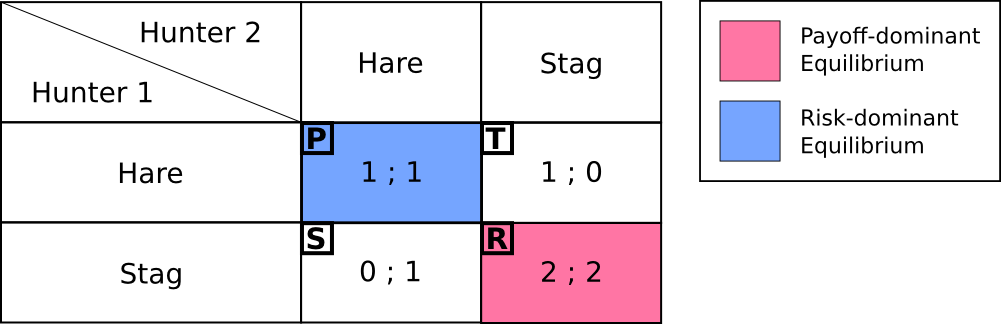
\includegraphics[scale = 0.50]{fig/Intro/StagHunt.png}
          \caption{\textbf{Matrice des gains de la chasse au lièvre.}
          Dans le jeu de la chasse au lièvre~\parencite{Skyrms2004}, on considère que durant une chasse, deux chasseurs peuvent soit chasser un lièvre ou un cerf. Chasser un lièvre peut être fait seul et assure l'obtention d'une récompense. En comparaison, chasser un cerf ne peut être fait que de manière coopérative mais rapporte plus qu'un lièvre. Par conséquent, un individu chassant un cerf seul n'obtiendrait aucune récompense. Les gains sont données de la manières suivante (Gain pour le chasseur 1; Gain pour le chasseur 2). Les valeurs exactes des gains n'ont pas d'importance tant que les différentes situations sont dans l'ordre suivant: R (récompense de la coopération) > T (tentation de tricher) = P (punition d'avoir triché) > S (sucker's payoff, c'est-à-dire la punition de s'être fait avoir). L'équilibre appelé "payoff-dominant" est l'équilibre où les chasseurs maximisent leur gain maximum tandis que l'équilibre appelé "risk-dominant" est celui où ils maximisent leur gain minimum.} 
          \label{fig:MatrixStagHunt}
        \end{center}
    \end{figure}


  \subsection{Robotique Evolutionniste}

    \begin{figure}[hbt]
        \begin{center}
          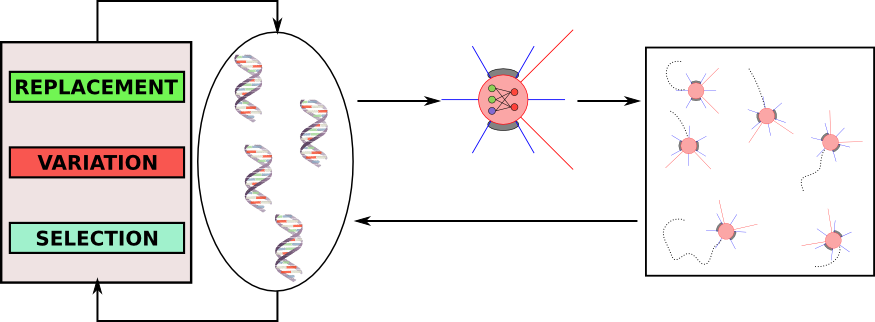
\includegraphics[scale = 0.50]{fig/Intro/EvolutionaryRobotics.png}
          \caption{\textbf{Fonctionnement général d'un algorithme de robotique évolutionniste.}
          Le but principal de l'ER est d'évoluer une population de génotypes. A cette fin, chaque génotype doit être évaluté afin d'obtenir un score de fitness. Un génotype est traduit en phénotype (ici un réseau de neurones artificiels) et ensuite intégré dans un robot afin d'agir en tant que contrôleur. Le robot situé dans son environment et son comportement est évalué en fonction des spécificités de la tâche. Une fois qu'on a assigné à chaque génotype un score de fitness, on utilise un algorithme évolutionniste. Cette phase sélectionne les génotypes jugés aptes à créer des descendants sur lesquels on applique de la variation. Finalement, cette nouvelle population de génotypes remplace la population précédente et le processus peut continuer pour une nouvelle génération.} 
          \label{fig:EvolutionaryRobotics}
        \end{center}
    \end{figure}

    Dans le contexte de cette thèse, le problème des modèles en théorie des jeux est qu'ils font des hypothèses que nous jugeons critiques sur les mécanismes proximaux. En particulier, il est généralement supposé qu'une mutation seule est suffisante pour évoluer un comportement coopératif pour un individu initialement non coopératif. Cela veut donc dire qu'une hypothèse est faite sur la disponibilité des mutations. Dans notre cas, puisque nous souhaitons étudier l'amorçace de la coopération mutualiste et le rôle de la coordination dans cette évolution, nous pensons que faire cette hypothèse masque l'influence des mécanismes proximaux sur l'évolution de la coopération. C'est pourquoi nous choisissons d'utiliser une méthode particulière pour aborder notre problème : la \emph{robotique évolutionniste} (ou ER).

    Le principe de la robotique évolutionniste est à la base de concevoir des robots en appliquant des concepts inspiré de l'évolution naturelle. Plus précisément, l'idée est d'appliquer des processus de sélection et de variation afin de pouvoir concevoir automatiquement des robots avec une approche holistique~\parencite{Nolfi2000, Doncieux2015a}. Le fonctionnement classique d'un algorithme d'ER est résumé dans la Figure~\ref{fig:EvolutionaryRobotics}. Concrètement, le but de l'ER est d'évoluer une population de génotypes. La forme exacte du génotype est extrêmement variable en fonction des travaux mais un choix courant est d'utiliser une liste de nombres réels. Ce génotype est alors traduit en un phénotype. Une fois encore, les formes des phénotypes sont très variables. Le point important est que ce phénotype est intégré dans un agent robotique (réel ou simulé) et permet de représenter le ou les traits du robot que nous souhaitons faire évoluer, que ce soit sa morphologie ou son contrôle. Par exemple, une implémentation courante de phénotype dans le cas du contrôle d'un robot est d'utiliser un réseau de neurones artificiels. Le robot est alors évalué dans un environnement afin d'accomplir une certaine tâche. Sa performance par rapport à cette tâche est ce qui détermine son score de fitness. 

    Une fois chaque génotype évalué vient l'étape de l'algorithme évolutionniste qui permet de créer la population de génotypes de la génération suivante. Pour celà on sélectionne d'abord les génotypes qu'on considère aptes à pouvoir se reproduire. Ces génotypes sont alors copiés afin de créer des descendants. Ensuite, on applique de la variation sur les descendants créés, ce qui peut consister en de la mutation et/ou de la recombinaison. Une fois cette étape passée, ces génotypes constituent la population de la nouvelle génération et on peut entamer une nouvelle génération comme précédemment.

    Le point important de la robotique évolutionniste est qu'on évalue directement les phénotypes résultant de l'évolution des génotypes des individus. Cette technique peut donc être utilisée pour observer et étudier les comportements évolués ainsi que leurs intéractions avec un environnement aux conditions écologiques précises. En particulier, l'ER permet de faire le minimum de suppositions quand à la disponibilité des mutations et ainsi de pouvoir étudier en détail l'influence des mécanismes proximaux sur l'évolution de la coopération.


   \subsection{Setting Expérimental}

   	Maintenant que nous avons clairement posé nos hypothèses de travail, nous pouvons présenter notre setting expérimental. Nous choisissons donc de modéliser le problème de la chasse au cerf avec des techniques de robotique évolutionniste. Pour celà, nous étudions l'évolution de comportements coopératifs chez des agents robotiques \emph{simulés}. Chaque agent robotique est capable de mouvement et est équipé de deux type de senseurs différents. D'abord chaque agent est équipe d'une caméra frontale à $90$ degrés. Cette caméra permet de reconnaître le type de chaque objet (y compris les autres agents) qu'elle voit dans l'environnement ainsi que de renseigner sur leur proximité. Ensuite les agents possèdent aussi $12$ senseurs de proximités répartis tout autour de leur corps et qui permettent de ressentir les obstacles autour d'eux.

   	Chaque robot est contrôlé par un réseau de neurones artificiels. Ce réseau est un perceptron multi-couches avec une couche cachée et entièrement connecté. Les entrées du réseau sont constituées de l'ensemble des informations sensorielles de l'individu. Etant donné un ensemble d'entrées, le réseau de neurones permet de calculer deux valeurs de sortie qui correspondent aux vitesses respectives de chacune des deux roues du robot, permettant ainsi le déplacement.

   	L'environnement dans lequel évolue les robots est une arêne carrée entourée de $4$ murs. Cette arêne est remplie d'un certain nombre de proies qui peuvent être de type différent. Notamment, ces proies permettent de représenter les lièvres et cerfs qu'un chasseur peut chasser dans le modèle de la chasse au cerf. Tandis que ces proies sont immobiles, les agents robotiques peuvent se déplacer librement dans l'environnement. Afin d'attraper une proie, il est nécessaire pour un robot de rester au contact de cette proie pendant un temps prédéfini. Une fois ce temps passé, la proie est retirée et replacée à un endroit aléatoire de l'arêne afin de conserver la même proportion de proie durant toute une simulation. L'individu ayant chassé la proie reçoit alors une récompense dépendant de la proie et de si elle a été chassée de manière solitaire ou collective. Afin de chasser de manière collective, il est nécessaire aux deux individus de se trouver au contact de la proie au moment où elle est retirée de l'environnement. Ceci veut donc dire qu'il est nécessaire aux individus d'évoluer des comportements de coordination afin de pouvoir effectivement coopérer

   	Le génotype d'un individu correspond aux poids des connexions du réseau de neurones. Nous ne faisons pas évoluer la topologie du réseau. Afin d'évoluer les génotypes, nous utilisons un algorithme évolutionniste classique. L'évolution commence avec une population de génotypes initialisés aléatoirement. Afin d'évoluer chaque individu, cet individu est apparié avec un autre individu tiré aléatoirement dans la population. Ces deux individus sont alors évalués dans l'arêne présentée précédemment. Afin de diminuer les effets stochastiques dus au placement initial aléatoire des proies, $5$ simulations indépendantes sont effectuées pour chaque paire. Afin que chaque individu rencontre un échantillon représentatif de la population, l'individu évalué est au total apparié avec $5$ individus différents. Une fois que tous les individus ont été évalués, les génotypes sont sélectionnés en fonction de deux processus de sélection différent selon l'expérience : une stratégie élitiste \((\mu+\lambda)\)-ES ou \emph{fitness proportionate}. Dans le premier cas, on parle de stratégie éliste car les meilleurs individus de la génération sont conservés pour la génération suivante. Plus précisément, on sélectionne les $\mu$ meilleurs individus (en terme de score de fitness) qui sont alors directement transférés dans la population de la prochaine génération. On crée alors $\lambda$ descendants à partir de ces $\mu$ meilleurs individus. Dans le cas du \emph{fitness proportionate}, le processus de sélection est plus proche du processus naturel de la sélection naturelle. En effet, afin de créer chacun des descendant constituant la nouvelle génération, on sélectionne aléatoirement parmi la population de parents (donc la population de la génération courante). Cependant, chaque parent a une probabilité plus forte d'être sélectionné si son score de fitness relatif par rapport aux autres individus de la population est plus élevé. Quelque soit la méthode de sélection, chaque descendant est un clone de son parent sur lequel on applique des mutations aléatoires. Ceci veut donc dire que nous n'utilisons pas de recombinaison.


\section{Modélisation de l'Evolution de la Coopération en Robotique Évolutionniste}

	\subsection{Motivation de la méthode}
	
		Dans une première partie de la thèse, nous sommes intéressé par la modélisation computationnelle de l'évolution de la coordination. Plus particulièrement, nous souhaitons utiliser des outils de robotique évolutionniste afin d'étudier l'influence des comportements de coordination dans l'évolution de la coopération mutualiste. En effet, comme expliqué dans l'introduction, les mécanismes proximaux ont souvent été ignorés quant à l'étude de ce type de comportement coopératif. Pourtant, ce sont ces mécanismes qui ont une influence sur la disponibilité des mutations vers la coopération. Plus précisément, nous pensons que dans les modèles classiques pour l'étude de l'évolution de la coopération, des hypothèses critiques sont faites et qui peuvent réellement changer la complexité de l'évolution des comportements collectifs.

		Nous choisissons d'utiliser de la robotique évolutionniste car cette méthode permet en effet de considérer en détail les explications proximales par rapport à d'autres méthode plus classique en biologie évolutionniste. Par exemple comme nous l'avons précédemment dit une méthode très classique pour étudier l'évolution de la coopération est d'utiliser de la théorie des jeux évolutionniste. Cependant, dans ce type de modèles, il est souvent considéré qu'une mutation seule permet d'évoluer la coopération pour un individu se comportant de manière solitaire. En pratique, l'évolution de la coopération sous-entend dans notre cas l'évolution de la coordination et donc d'un comportement complexe avant que des individus soient capables de récolter les bénéfices d'une action coopérative. Il est donc nécessaire d'utiliser une méthode qui nous permette d'étudier ces mécanismes avec précision.

		Pour celà, il est nécessaire de se tourner vers les méthodes de modélisation individu-centré (IBM)~\parencite{Huston1988}. Ces méthodes permettent de modéliser finement le comportement des individus et ensuite de s'intéresser à l'influence qu'ont les intéractions individuelles sur le comportement collectif. Ce type de modèles s'intéresse donc à la modélisation des variations individuelles et permet ainsi de minimiser le nombre de suppositions faites à ce niveau-là~\parencite{Adami2014}. De ce fait, un certain nombre de travaux ont été intéressé par la modélisation de phénomènes biologiques à l'aide d'IBM : de la formation des troupeaux~\parencite{Olson2013a, Haley2014, Olson2016} à l'évolution de l'altruisme~\parencite{Wilder2015} en passant par la symbiogénèse~\parencite{Watson1992}.

		Dans notre cas, nous pouvons considérer la robotique évolutionniste comme une instance particulière d'IBM. Les deux méthodes s'intéressent en effet à la modélisation des individus dans le but de l'étude d'une émergence collective. Un certain nombre de travaux en IBM utilise en fait le paradigme de l'ER. Mais le principal atout de l'ER par rapport aux IBM est le fait que l'individu soit incarné~\parencite{Mitri2012} (un concept équivalent à celui \emph{d'embodiment}). Les robots ont un corps physique ce qui rajoute un niveau supplémentaire d'intéractions. En comparaison, on fait parfois abstraction de ce genre de concepts en IBM. Or, l'embodiment peut justement avoir des effets inattendus et intéressants sur l'évolution de comportements collectifs~\parencite{Mitri2009}. Nous choisissons donc ici d'utiliser la robotique évolutionniste dans le but d'avoir ce niveau de modélisation supplémentaire et d'encore réduire le nombre de suppositions sur les mécanismes du comportement que nous faisons. Il est à noter que, même si de nombreux travaux récents se sont intéressés à l'utilisation de la méthode ER pour la modélisation de l'évolution de la coopération~\parencite{Waibel2009, Waibel2011, Montanier2011, Ferrante2015}, l'évolution de la coopération mutualiste a en grande partie été ignorée de cette littérature.


	\subsection{Résultats}

		\subsubsection{L'Influence des mécanismes du comportement sur l'évolution de la coopération}

			Les premiers résultats présentés dans cette thèse sont centrés sur l'impact des mécanismes proximaux sur l'évolution de la coopération mutualiste. Ces résultats ont été publiés dans un journal international :

			\begin{quote}
			  \fullcite{Bernard2016a}
			\end{quote}

			Notre but est de montrer que les mécanismes des comportements de coordination sont critiques dans l'évolution des actions collectives. En particulier, nous nous intéressons à l'évolution des comportements mutuellement bénéfiques. Comme expliqué précédemment, les comportements mutualistes sont stables une fois qu'ils ont été évolués parce qu'ils bénéficient tous les individus. Cependant, leur amorçage n'est pas évident parce que ces comportements souvent requièrent l'évolution de la coordination. Par conséquent, un individu seul ne peut bénéficier de la coopération à moins que d'autres ne coopèrent aussi.

			Nous nous inspirons ici d'un modèle de théorie des jeux appelé le stag hunt~\parencite{Skyrms2004}. Nous pensons que des suppositions critiques sont faites dans les modèles classiques de théorie des jeux qui pourrait cacher la complexité d'évoluer des actions mutualistes. En particulier, il est généralement supposé qu'une seule mutation est suffisante pour évoluer un individu coopératif à partir d'un individu solitaire. En réalité, l'évolution de la coopération implique l'émergence de plusieurs traits qui ne pas sont bénéfiques par eux-mêmes. Nous pensons ainsi que des contraintes mécanistiques critiques sur l'évolution de la coordination ont été négligées par ces modèles classiques. Afin de prendre ces mécanismes en compte, nous modélisons le stag hunt en robotique évolutionniste~\parencite{Nolfi2000, Doncieux2015}. Deux individus sont évolués dans une arêne fermée remplie de $18$ proies, la moitié d'entre elles étant des lièvres, l'autre moitié des cerfs. Chasser un lièvre rapporte moins que de chasser un cerf et peut être accompli de manière solitaire ou coopérative. En comparaison, les bénéfices de la chasse d'un cerf ne peuvent pas être obtenus à moins que les deux individus tuent la proie ensemble.

			Nous révélons alors qu'il existe des différences drastiques lorsque la transition vers la chasse au cerf est modélisée en robotique évolutionniste. En particulier, nous montrons que l'évolution de l'équilibre coopératif (la chasse au cerf) lorsque les individus agissent initiallement de manière solitaire (chasser au lièvre) apparait toujours avec un modèle en théorie des jeux classique. En comparaison, en robotique évolutionniste l'amorçage de la coopération est presque impossible puisque cette transition n'apparaît que dans $1$ réplicat sur $30$. De plus, même quand les individus sont génétiquement proches, la transition vers la coopération est toujours peu probable puisqu'elle n'apparait que dans 20\% de tous les réplicats. Notre modèle révèle ainsi que la transition vers la coopération est confrontée à un dilemme de l'oeuf et de la poule. Plus précisément, la coopération ne peut pas être sélectionnée à moins qu'elle ne soit bénéfique pour l'individu. Mais les bénéfices de la coopération ne peuvent être obtenus à moins que d'autres individus ne soient capable de coordination. En particulier, nous observons que l'évolution de la coordination implique l'émergence d'un comportement complexe qui a peu de probabilité d'évoluer. Par conséquent, nous démontrons que les mécanismes pratiques de la coordination ont un impact critique sur l'évolution de la coopération mutuellement bénéfique. Nous soutenons donc que les modèles considérant les expliquations proximales de la coopération sont nécessaires afin d'avoir une compréhension complète de l'évolution de la coopération mutualiste.


		\subsubsection{Optimisation des actions collectives par le biais de la sélection individuelle}

			Nous avons révélé à l'aide des résultats précédents que l'évolution des actions collectives était entravée par l'évolution de la coordination. En particulier, nous avons utilisé la robotique évolutionniste afin de mettre en lumière les contraintes mécanistiques qui agissent sur la transition d'un équilibre solitaire vers un équilibre coopératif. Notre intérêt a alors ensuite été de comprendre comment la sélection individuelle pouvait permettre la transition entre différents équilibres collectifs

			Les actions collectives permettent d'obtenir des bénéfices grâce aux intéractions de plusieurs individus. Même dans le cas où ces actions bénéficient à tous les individus de manière mutualiste, il n'est pas bien compris comment ces comportements collectifs sont atteint. Plus précisément, puisqu'ils requièrent la coordination de multiples individus, plusieurs équilibres évolutionnistes stables peuvent émerger. Mais, parce que les bénéfices sont obtenus par une action collective, un individu seul s'écartant de l'équilibre évolué ne serait pas adaptatif. Ceci veut dire qu'un mutant agissant vers un équilibre différent ne sera pas sélectionné, même si cet équilibre pourrait s'avérer plus avantageux pour le groupe. Par conséquent, ceci pose le problème de l'optimisation des actions collectives. A savoir, comment est-il possible pour la sélection individuelle d'amener à la transition vers un équilibre optimal quand un autre équilibre collectif a déjà évolué.

			Un mécanisme classique pour résoudre ce problème est la sélection de groupe. Puisque ces comportements sont bénéfiques au niveau du groupe alors ceci impliquerait qu'ils sont sélectionnés au même niveau. Cependant, nous voulons étudier comment les comportements collectifs pourraient être optimisés par la sélection individuelle uniquement. A cette fin, nous choisissons de modéliser l'exemple de la chasse collective. En particulier, nous utilisons un modèle similaire à celui de nos précédents résultats. A savoir, des individus sont évolués dans un environnement où ils peuvent chasser deux types de proies aux récompenses différentes: \emph{sanglier} et \emph{cerf}. Chaque type de proie correspond à un équilibre collectif différent: sous-optimal pour le sanglier et optimal pour le cerf. Notre but est ainsi d'étudier la transition de l'équilibre sous-optimal (chasse au sanglier) vers l'équilibre optimal (chasse au cerf).

			Nous montrons que sous des caractéristiques écologiques simples où seulement des proies sont présentes dans l'environnement, la transition vers l'optimum est impossible. Cependant, dans le contexte de suppositions plus réalistes où les individus doivent choisir entre plusieurs proies, alors l'équilibre optimal est évolué dans $8$ réplicats sur $30$. En particulier, les individus doivent maintenant se coordonner afin de réussir à coopérer. Celà veut dire qu'ils doivent réagir au comportement de l'autre. De là il découle qu'ils réagissent aussi au comportement d'un mutant. Ceci permet donc en retour au groupe de bénéficier de la chasse au cerf.

			Cependant, dans la stratégie de coordination précédemment évoluée, les deux individus choisissent séparément quelle proie chasser. Nous étudions alors comment une stratégie de coordination plus asymétrique pourrait impacter la transition vers l'optimum. A cette fin, nous augmentons la complexité des réseaux de neurones contrôlant les individus afin de leur permettre d'évoluer des stratégies de coordination plus complexes. Dans ce cas, nous révélons que la transition vers l'optimum est facilitée puisque la chasse au cerf évolue dans $24$ réplicats sur $30$. De plus, nous observons l'évolution d'une stratégie asymétrique plus efficace où les individus adoptent deux rôles différents : la stratégie de \emph{leader/suiveur}. Dans cette stratégie, seul le leader décide de quel proie chasser le suiveur se contentant d'aller sur la même proie. Par conséquent, alors que choisir de coopérer sur un cerf était précédemment un problème de décision collective, il s'agit maintenant d'un problème individuel. Celà veut dire qu'un leader mutant allant vers un cerf est maintenant suffisant pour que les deux individus récoltent les bénéfices de la chasse au cerf. De plus, la stratégie de leader/suiveur a évolué parce qu'elle est plus efficace. Nous avons ainsi montrer que l'évolution d'une stratégie de coordination individuellement adaptative a mené vers l'optimisation d'un comportement collectif.



\section{Conception de Robots Coopératifs}

	\subsection{La Robotique Évolutionniste pour la Conception de Robots}

		Dans la seconde partie de la thèse, nous nous intéressons cette fois à la conception de robots coopératifs. Plus précisément, notre but est de s'inspirer de ce que nous avons appris grâce à nos résultats sur la modélisation biologique afin de permettre l'évolution de robots capable de coopérer. En particulier, nous voulons permettre l'évolution de la coopération entre robots hétérogènes.

		Les systèmes multi-robots (MRS) ont plusieurs avantages en comparaison d'un seul robot. Par exemple, ils peuvent permettre de résoudre plus facilement et/ou plus rapidement une tâche qu'avec un seul robot. Ils permettent aussi d'assurer plus de robustesse de la part du système puisque la présence de multiples robots peut être utilisée pour éviter que l'ensemble du système soit compromis suite à la panne d'un seul de ses élements. Il peut parfois aussi être plus rapide et moins coûteux de concevoir plusieurs robots aux capacités simples plutôt qu'un unique robot complexe. Mais concevoir un MRS est complexe. Il est en effet nécessaire d'être capable de concevoir le contrôle de plusieurs robots dont on s'attend à ce qu'ils fonctionnent simultanément. En particulier, de nombreuses caractéristiques de conception rentrent en compte dans la façon dont on va créer un MRS: centralisé/distributé, robots homogènes/hétérogènes, nombre de robots. 

		Les méthodes utilisées pour créer ces MRS dépendent principalement des choix fait à propos de ces caractéristiques architecturales. Depuis la création de ce domaine, de nombreuses méthodes ont été proposées, notamment afin de résoudre le problème du contrôle d'un MRS. Historiquement, les premières approches ont consisté à coder directement le comportement des robots afin d'obtenir le résultat désiré. Ceci a été très inspiré par les techniques appliquées sur des robots uniques et le but a souvent été d'adapter ces techniques pour plusieurs robots. Néanmoins, le contrôle d'un MRS est très différent d'un seul robot et souvent coder directement le comportement des individus devient beaucoup plus compliqué. Par exemple, il faut être capable d'anticiper l'émergence d'un comportement collectif à partir d'un ensemble de comportements individuels, impliquant beaucoup d'allers-retours afin d'atteindre le comportement désiré.

		Il y a donc eu assez vite un intérêt pour utiliser des méthodes d'apprentissage afin d'automatiser la conception de MRS. Ainsi, de nombreux travaux se sont intéressés à utiliser de l'apprentissage par réinforcement (RL)~\parencite{Sutton1998}  dans ce but. Il existait déjà une grande littérature à ce sujet pour la conception automatique de robots seuls et là encore le but a été d'adapter ces techniques pour les MRS~\parencite{Gultekin2002, Bowling2003, Fernandez2005}. Mais appliquer des techniques d'apprentissage à plusieurs robots est complexe. En particulier, ceci implique souvent de simplifier le problème et d'utiliser des approximations afin d'être capable de pouvoir adopter ces algorithmes aux MRS.

		En comparaison, la robotique évolutionniste possède de nombreux avantages par rapport à l'apprentissage par renforcement. En particulier, il n'y a pas besoin d'estimer l'espace des états ce qui fonctionne très bien pour les problèmes en environnement ouvert et en boîte noire. Par conséquent, de nombreux travaux se sont intéressés à l'ER pour les MRS~\parencite{Watson2002, Brambilla2012, Hauert2014, Francesca2016}. En particulier, un problème intéressant pour la conception de MRS en ER est le fait de choisir entre des groupes de robots homogènes ou hétérogènes~\parencite{Waibel2009}. Des robots homogènes sont plus simples à évoluer puisque tous les robots bénéficient de la coopération. En comparaison, des équipes hétérogènes permettent d'avoir accès à une plus grande diversité de comportements entre les individus et donc potentiellement à des technique de coordination plus efficaces. Mais si les groupes sont hétérogènes alors ceci crée le problème de l'évolution de la coopération et du fait que des individus peuvent agir de manière égoiste. Dans cette partie de la thèse nous nous intéressons donc à l'évolution des comportements de coordination parmis un groupe de robots hétérogènes.

	\subsection{Résultats}

		\subsubsection{Le compromis entre évolvabilité et efficacité en robotique évolutionniste}

			Notre première étude dans cette partie de la thèse est concentrée sur l'évolution des comportements de coordination dans une tâche de récolte collective. Ces résultats ont été publié dans une conférence internationale :

			\begin{quote}
			  \fullcite{Bernard2015}
			\end{quote}

			Nous sommes intéressés par le sujet d'évoluer de la coopération parmi un groupe de robots hétérogènes. En particulier, nous souhaitons comparer une approche homogène (que nous appelons ici approche clonale) et une approche hétérogène. L'approche la plus classique pour concevoir des MRS en robotique évolutionniste est d'utiliser des groupes de robots homogènes. C'est en effet la manière la plus sûre de s'assurer de l'évolution de la coopération parce que la fitness des agents est la même que celle du groupe. Cependant, cela veut dire que nous nous concentrons souvent sur \emph{l'évolvabilité} de la coopération, c'est-à-dire la probabilité d'évoluer des individus coopératifs~\footnote{Il est important de préciser que le terme "évolvabilité" a une forte connotation dans le domaine de la robotique évolutionniste et qu'il peut correspondre à plusieurs définitions. En particulier, une de ces définitions est que l'évolvabilité représente la capacité pour un individu de s'adapter aux changements dans l'environnement~\parencite{Wagner1996}. Il s'agit d'un sujet prometteur en évolution artificielle~\parencite{Banzhaf2006, Lehman2013, Doncieux2015a, Taylor2016} et par conséquent nous ne voulons pas créer de confusion quant à notre utilisation du terme. Dans cet article, l'évolvabilité fait uniquement référence à la capacité d'évoluer un trait particulier (dans notre cas la coopération)}. Cependant des groupes de robots hétérogènes peuvent permettre d'atteindre une plus grande \emph{efficacité} (en terme de fitness) quand de la coordination est nécessaire. Parce que les individus peuvent adopter des comportements distincts, ils peuvent évoluer des stratégies de coordination plus diverses. Mais la présence d'hétérogénéité peut aussi gêner l'évolution de la coopération dans un environnement où il est possible pour les robots de se comporter de manière égoiste. Nous voulons ainsi comparer ces deux approches dans ce genre d'environnement sur la base de deux critères : évolvabilité et efficacité.

			A cette fin, nous avons conçu une tâche de recolte collective inspirée par le stag hunt. Plus précisément, deux individus sont placés dans une arêne où ils peuvent collecter deux types différents de ressources : vert et violet. Les ressources vertes rapportent autant qu'elles soient collectées de manière solitaire ou collective. En comparaison, les ressources violettes doivent être collectées coopérativement mais rapportent plus que les vertes. Etant donné cette tâche, nous étudions l'évolution de comportements coopératifs, c'est-à-dire quand les individus collectent ensemble des ressources violettes. Nous étudions trois compositions de groupes différentes :

			\begin{itemize}
			  \item{Contrôle, où les individus viennent de la même population mais sont génétiquement différents.}
			  \item{Clonal, où les individus sont des clones l'un de l'autre.}
			  \item{Coévolution, où les individus viennent de populations différentes.}
			\end{itemize}

			Nous comparons alors les résultats de deux approches hétérogènes (contrôle et coévolution) et d'une approche clonale sur les deux critères présentés précédemment.

			Nous révélons qu'il existe un compromis entre évolvabilité et efficacité dans notre tâche de récolte. En particulier, l'approche clonale donne les meilleurs résultats pour ce qui est d'évoluer des individus coopératifs. En comparaison, l'approche en coévolution permet l'émergence de comportements coopératifs plus efficaces. De plus on observe, dans l'approche en coévolution, l'évolution de division du travail par le biais d'une stratégie de \emph{leader/suiveur}. Nous souhaitons alors dépasser ce compromis et améliorer chacune des approches sur les deux critères d'évolvabilité et d'efficacité.

			Pour celà, nous utilisons de l'évolution incrémentale. Les individus sont d'abord pré-évolués dans une tâche de coopération plus simple où ils doivent traverser un ensemble de points de passage. Les individus sont récompensés par le fait de traverser les mêmes points de passage dans le même ordre. Après ça, ces individus sont évolués dans la tâche de collecte présentée précédemment. Nous montrons que, bien que la probabilité d'évoluer la coopération augmente sous coévolution, aucun différence significative n'est observée avec l'approche clonale. Ceci veut alors dire que l'approche en coévolution atteint les meilleurs scores d'évolvabilité \emph{et} d'efficacité comparé aux autres approches. Nous montrons alors qu'il existe un nouveau compromis : il est possible d'améliorer l'évolvabilité de stratégies de coordination efficaces mais au coût de temps computationnel supplémentaire.


		\subsubsection{L'évolution de la spécialisation dans une population de robots hétérogènes}

			Nous étudions maintenant l'évolution de la division du travail entre des robots hétérogènes par le biais de polymorphisme génotypique. Ces résultats ont été publiés dans une conférence internationale :

			\begin{quote}
			  \fullcite{Bernard2016b}
			\end{quote}

			Nous avons précédemment montré qu'il pouvait être bénéfique de considérer la qualité des comportements de coopération en plus de la probabilité d'évoluer la coopération. En particulier, nous avons montré qu'une approche hétérogène particulière, la coévolution coopérative, permettait l'émergence d'une stratégie de coordination plus efficace: leader/suiveur. Ce comportement implique l'évolution de spécialisation (ou division du travail). Ici nous nous intéressons à l'évolution d'une stratégie de leader/suiveur dans une seule population d'individus

			Puisque la coopération est souvent atteinte entre robots homogènes en robotique évolutionniste, alors pour permettre de la division du travail les individus doivent être capable d'adapter leur phénotype durant leur vie. Par conséquent, la spécialisation repose sur de la plasticité phénotypique ou des informations environnementales. Ici nous nous sommes intéressés par l'évolution de la spécialisation sans ces mécanismes supplémentaires. Ceci veut dire que nous voulons créer de la division du travail au niveau de la population. Par conséquent, nous voulons étudier le maintien de plusieurs génotypes différents codant pour différent rôles dans une unique population, c'est-à-dire du polymorphisme génotypique. En particulier, nous nous concentrons sur l'impact des méthodes de séléction sur l'évolution du polymorphisme génotypique.

			A cette fin, nous utilisons une tâche de récolte plus simple que celle utilisée précédemment. Deux individus génétiquement différent sont placés dans une arêne où ils peuvent récolter un seul type de ressource. Cette ressource est plus intéressante si elle est récoltée de manière coopérative. Ceci veut dire qu'évoluer la coopération est simple (ce n'est pas le sujet ici) et que l'accomplissement de la tâche est favorisé par l'évolution de stratégies de coordinations efficaces. Comme montré dans les résultats précédents, deux stratégies de coopération différentes peuvent évoluer dans cette tâche. D'un côté, il y a la stratégie des \emph{tourneurs}, où les deux individus adoptent le même comportement afin de se coordonner. Il s'agit donc d'une stratégie généraliste. D'un autre côté, ils peuvent aussi évoluer des comportements de spécialistes et adopter une stratégie de \emph{leader/suiveur}. Nous nous intéressons à l'étude des différences évolutionnaires de deux méthodes de sélection différentes: (1) un \((\mu + \lambda)\)-ES (sélection élitiste) et (2) une sélection fitness-proportionate. Nous étudions aussi l'impact de la taille de la population.

			Nous révélons que la spécialisation est presque impossible à évoluer quand une sélection élitiste est utilisée. En effet, dans un seul réplicat sous grande taille de population nous observons la présence de spécialistes dans la population à la fin de l'évolution. De manière surprenante des spécialistes apparaissent néanmoins dans plusieurs réplicats mais ne sont jamais maintenus. Même lorsque la population est initialisée avec des spécialistes des résultats similaires sont observés. En comparaison, tandis que les spécialistes ne sont presque jamais évolués en sélection fitness-proportionate, ils sont facilement maintenus durant l'évolution (en particulier quand la population est initialisée avec des spécialistes). Nous révélons ainsi que l'évolution de polymorphisme génotypique est gênée par le défi à la fois d'évoluer et de maintenir des spécialistes dans la population et qu'aucune de nos deux méthodes de sélection n'est appropriée pour celà.

			Nous utilisons alors des analyses computationnelles afin de mieux comprendre les mécanismes sous-jacent à ce problème. Nous montrons que bien que les spécialistes soient les plus efficaces, les généralistes peuvent envahir la population parce qu'ils ont de bons résultats contre n'importe quel phénotype. En comparaison, les spécialistes ont besoin d'être appariés avec d'autres spécialistes d'un type différent pour avoir les meilleurs résultats. Des analyses complémentaires montrent que, sous une taille de population finie, la diversité génétique peut être perdue d'une génération à l'autre. Nous révélons ainsi deux propriétés critiques pour l'évolution du polymorphisme génotypique: (1) la protection contre l'invasion de généralistes et (2) le maintien de la diversité génotypique. Nous soutenons qu'un algorithme possédant ces propriétés pourrait permettre d'obtenir du polymorphisme génotypique.


\section{Conclusions}

	\subsection{Contributions}

		Dans cette thèse nous avons abordé le sujet de l'évolution de la coordination en robotique évolutionniste. Pour cela, nous avons pris deux approches différentes liées à la robotique évolutionniste~\parencite{Nolfi2000, Doncieux2015a} : la modélisation et la conception~\parencite{Trianni2014b}.

		Pour la première approche, nous nous sommes intéressés à modéliser l'évolution de la coopération mutualiste en robotique évolutionniste. Plus précisément, nous avons utilisé des outils de cette méthode afin de pouvoir étudier l'influence des mécanismes proximaux de la coordination sur l'évolution de la coopération. Pour celà, nous avons pris inspiration du modèle de théorie des jeux du stag hunt~\parencite{Skyrms2004} où des individus peuvent choisir de chasser des lièvres de manière solitaire ou de coopérer pour chasser des cerfs qui sont plus intéressants pour eux. Nous avons tout d'abord montré qu'en utilisant une méthode en robotique évolutionniste, il était possible d'observer des différences drastiques avec des modèles classiques de théorie des jeux. Notamment, alors qu'avec un modèle classique l'évolution de la coopération (chasse au cerf) était facile, elle est presque impossible avec une modélisation en ER. En particulier, nous montrons que l'évolution de la coopération suppose l'évolution de comportement de coordination complexes qui n'ont que peu de chance d'évoluer seuls. En effet, la coordination ne peut pas être bénéfique tant que les individus ne coopèrent pas et vice versa. Nous révélons donc que, grâce à une méthode de modélisation en robotique évolutionniste, il est alors possible d'appréhender plus finement l'impact des mécanismes pratiques du comportement sur l'évolution de la coopération.

		Nous nous sommes alors intéressés à l'optimisation d'actions collectives. En particulier, nous voulions étudier comment la sélection individuelle pouvait permettre la transition d'un comportement collectif sous-optimal à un comportement collectif optimal. A première vue en effet, ce problème d'optimisation, parce qu'il concerne un comportement de groupe, ne devrait pouvoir être résolu que par le biais de la sélection de groupe. Nous montrons alors qu'il est possible d'atteindre l'optimum grâce à la sélection individuelle uniquement. En particulier, nous révélons que la coordination, parce qu'elle permet de réagir au comportement d'autres individus, permet aussi de réagir au comportement de mutants et donc ainsi de permettre de modifier indirectement le comportement du groupe. La nature de cette coordination change aussi la facilité avec laquelle cette action collective est optimisée. Ainsi, nous montrons aussi que lorsque des comportements de coordination asymétriques sont évolués, alors la transition vers l'optimum est grandement facilité. Ces stratégies asymétriques sont de plus sélectionnées parce qu'elles sont plus efficace pour les individus. La sélection individuelle est donc suffisante pour expliquer l'optimisation d'un comportement collectif.

		Puis, dans le cadre de la deuxième approche, nous avons alors étudié la conception automatique de systèmes multi-robots grâce à la robotique évolutionniste. En particulier, nous nous sommes intéressés à l'évolution de robots coopératifs dans une tâche nécessitant de la coordination entre robots faisant parti d'un groupe hétérogène. Dans un premier temps, nous avons comparé des approches homogènes et hétérogènes et montré que, dans un environnement où il était possible d'avoir des comportements égoistes, l'approche homogène permettait d'évoluer plus facilement la coopération. Cependant, avec une approche hétérogène (la coévolution dans ce cas), il était possible d'évoluer des stratégies de coopération plus efficace et notamment de la division du travail. Nous révélons ainsi l'existence d'un compromis entre évolvabilité et efficacité. En utilisant de l'évolution incrémentale, nous sommes capable de dépasser ce compromis en augmentant la probabilité d'évoluer des stratégies coopératives parmis un groupe hétérogène. Nous créons cependant aussi un deuxième compromis. En effet, il est possible d'augmenter l'évolvabilité de l'approche hétérogène mais en contrepartie il est nécessaire de payer un surcoût computationnel.

		Enfin, nous nous sommes finalement intéressés à l'évolution du polymorphisme génotypique au sein d'une population de robots. Plus précisément, nous avons étudié l'évolution de la division du travail au sein d'un groupe hétérogène de robots en fonction de la méthode de sélection de l'algorithme évolutionniste. Nous avons alors montré que, sous une sélection élitiste il était presque impossible de maintenir des spécialistes dans la population mais facile de les évoluer. En comparaison, sous une sélection fitness-proportionate, le maintien de ces spécialistes était facile mais leur évolution difficile. Par le biais d'analyses computationnelles, nous avons pu montrer que les généralistes pouvaient envahir la population et remplacer les spécialistes parce qu'ils ne nécessitaient pas de se retrouver avec un phénotype particulier afin de pouvoir accomplir la tâche efficacement. De plus, des analyses supplémentaires ont montré que la taille de la population était nécessaire au maintien de la diversité génétique. Ainsi, nous avons révélé des propriétés critiques qui pouvaient permettre de concevoir un algorithme capable d'évoluer du polymorphisme génotypique.


	\subsection{Perspectives}

		D'un point de vue de la modélisation de la coopération, cette thèse ouvre des perspectives intéressantes que aurions souhaité étudié en détail. En particulier, l'évolution de la communication représente un sujet majeur dans l'étude des comportements sociaux. Il serait ainsi possible d'étudier comment des individus pourraient évoluer d'eux-mêmes des capacités de communication et comment la communication pourrait alors influer l'évolution de la coopération. Une autre perspective intéressante serait de changer de paradigme et d'étudier l'évolution de la coopération dans un contexte en-ligne et dirigé par l'environnement~\parencite{Montanier2011, Montanier2013}. Dans ces conditions, les robots sont directement évolués dans l'environnement et il n'y a pas de phase de sélection séparée. De plus, lorsque l'évolution est dirigée par l'environnement la fonction de fitness n'est plus donnée directement mais naît de la nécessité de rencontrer d'autres individus afin de pouvoir créer des descendants. Ceci pourrait avoir des conséquences intéressantes pour l'évolution de l'évolution de la coopération.

		Pour ce qui est de la conception de systèmes multi-robots, une perspective serait d'étudier l'évolution de la coopération sous d'autres conditions. Tout d'abord, toutes nos expériences ont été effectuées sur des robots simulés. Il pourrait être intéressant de voir si nos comportements évolués en simulation pourraient être facilement transférables sur des robots réels. Ceci permettrait de valider que nos simulations ne font aucune supposition critique sur la modélisation de l'environnement qui empêcherait d'obtenir les mêmes résultats dans le monde réel. Un autre point intéressant serait d'étudier le rajout d'un objectif de diversité~\parencite{Lehman2008, Doncieux2014}. En particulier, utiliser de l'optimisation multi-objectifs à la fois sur la performance et la diversité génotypique et/ou phénotypique pourrait notamment permettre de s'assurer de l'évolution de comportements de coopérations efficaces.